\tikzstyle{lay} = [draw=black!90, text width=\textwidth/3, text centered, anchor=north west]
\tikzstyle{mlay} = [lay, text width=\textwidth/6.225]
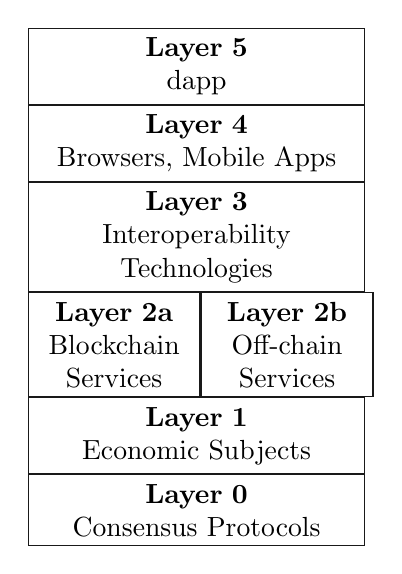
\begin{tikzpicture}
    \node (l5) [lay] {\textbf{Layer 5}\\\glspl{dapp}};
    \path (l5.south west) node [lay] (l4) {\textbf{Layer 4}\\Browsers, Mobile Apps};
    \path (l4.south west) node [lay] (l3) {\textbf{Layer 3}\\Interoperability Technologies};
    \path (l3.south west) node [mlay, anchor=north west] (l2a) {\textbf{Layer 2a}\\Blockchain Services};
    \path (l2a.east) node [mlay, anchor=west] (l2b) {\textbf{Layer 2b}\\Off-chain Services};
    \path (l2a.south west) node [lay] (l1) {\textbf{Layer 1}\\Economic Subjects};
    \path (l1.south west) node [lay] (l0) {\textbf{Layer 0}\\Consensus Protocols};
\end{tikzpicture}